\chapter{User Manual}
This manual will show how to execute Wazuh in the manager and agent in order to deploy or trobleshoot simple detection.

\section*{Requirements}
In order to execute the tools correctly a setup similar to this project is assumed.
Some elements may change without causing any differences in behaviour, but the recommendations are:
\begin{itemize}
	\item A Windows Server 2019 as the agent. It needs to install and configure the Wazuh agent with the manager. If the user wants other Windows machines in the network the recommendation is to configure AD and use it to set them up easier.
	\item A CentOS 7 running the ELK stack and the Wazuh manager. This can also have agent functionality for itself.
	\item All the computers or virtual machines in the same network, for optimal performance.
	\item Windows machines have Sysmon installed and configured to log the events of interest.
	\item The manager has been configured to make the agents forward the logs of interest to him.
	\item All the features of interest for the client have been configured.
\end{itemize}
\linej
In this case it is assumed that the agent is running on a Windows system.

\section*{Usage}
\subsection*{Basic detection of events}
If the format of the related events is unknown or if the events that should be generated are unknown, the user should force its execution and search the Windows Event Log (or the logs in \textit{/var/ossec/logs/archives/} if he is sure the events are forwarded to Wazuh).
The user may need to wait several minutes in order to see the event logged in Wazuh.
\linej
\linej
For fast debugging on how the event is processed by Wazuh the program logtest in \textit{/var/ossec/bin/ossec-logtest} can be used.
Several \textit{v} flags are recommended for more verbose.
To use it you only need to introduce the data as it would be received by the Wazuh manager.
It is possible to show which rules are tried and which trigger an alert for each event.
This tools does not need a restart of the wazuh-manager service whenever changes want to be tested because it reads the configuration directly.
\linej
But it is also worth to mention that some times it can be misleading because it does not work in the same way as the manager.
For example the logtest may show that the log matches a certain rule but actually it has matched a previous one silently.
\linej
\linej
For example for this input:
\linej

\includegraphics[width=\textwidth]{figuras/ossec-logtest_input.png}
\linej
We get the next output:
\begin{figure}[H]
  \centering
	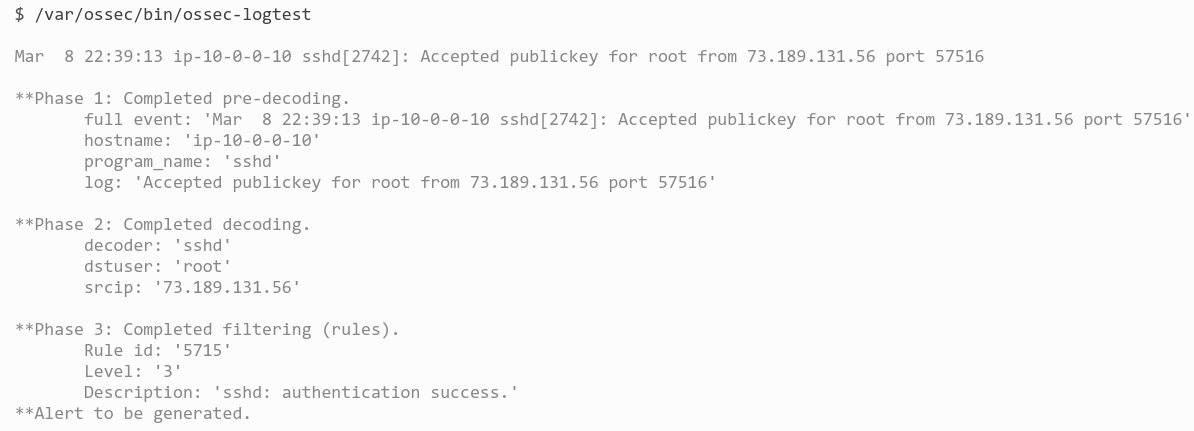
\includegraphics[width=\textwidth]{figuras/ossec-logtest_output.png}
	\caption{Example of output for ossec-logtest}
\end{figure}
\linej
This example shows how Wazuh processes the input text, that usually would be in a SSH event.
The decoder \textit{sshd} matches the format of the input text, and that it is able to extract the \textit{dstuser} and \textit{srcip} fields.
Then the event is processed by the set of rules until it matches the conditions of the rule 5715, which should generate an alert.
\linej
\linej
After identifying the desired detection the user can edit the rules in the file designed for custom rules \textit{/var/ossec/etc/rules/local\_rules.xml} to configure the alert logic desired.
Debugging the rules can be hard because Wazuh does not show why a rule does not trip.
The fastest way to find a way to match a rule for the desired condition is to write multiple slighty different rules and see which one is triggered.
\linej
\linej
For finding the alerts triggered the user can use a web browser to connect to the Kibana addon hosted by the manager, providing a graphical interface that allows to set multiple filters and that generates charts on the fly.
\begin{figure}[H]
  \centering
	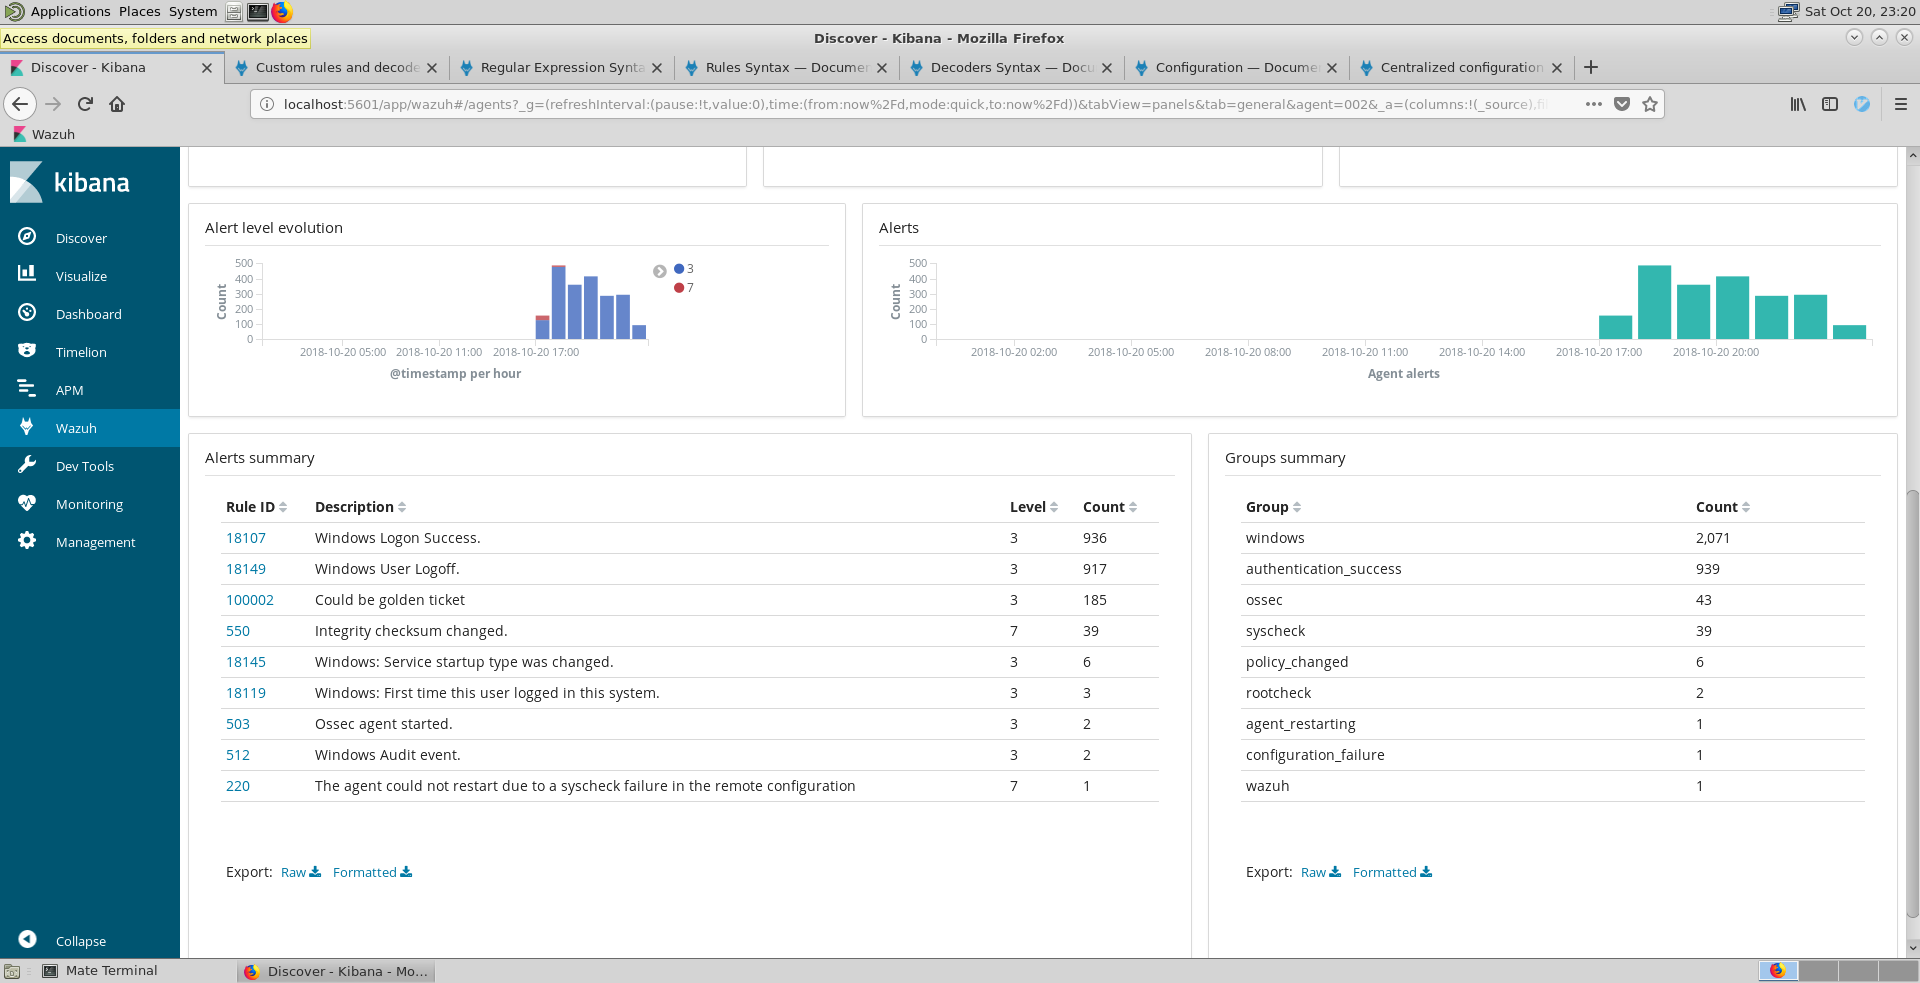
\includegraphics[width=\textwidth]{figuras/Kibana.png}
	\caption{Kibana showing the general view of the last alerts}
\end{figure}
\linej

Using commands directly on the log files is usually faster, but it may require expert knowledge to do it right.
This knowledge is basic if the user wants to be able to add custom functionality, like more monitoring options.
\begin{figure}[H]
  \centering
	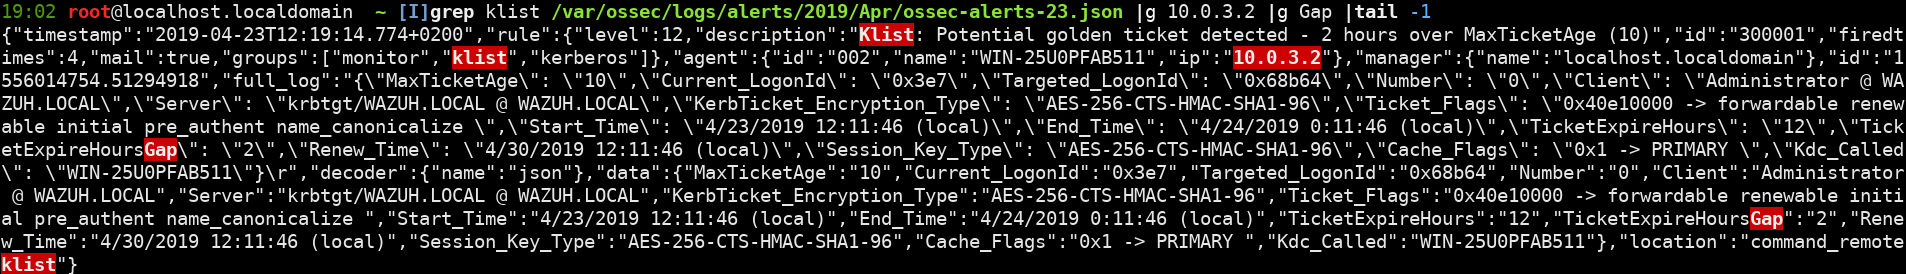
\includegraphics[width=\textwidth]{figuras/klist_alert.png}
	\caption{Latest alert of the klist custom monitoring in the manager}
\end{figure}

\subsection*{Dharma in a virtual machine}
To run the cmd version of Dharma in a virtual machine it is recommended to uninstall the virtual box guest additions (or similar software for your virtualization alternative).
Disabling network interfaces is also recommended, but it is not possible in this case because the ransomware needs to contact the C\&C.
The ransomware can be donwloaded from:
\begin{lstlisting}[style=txt,numbers=none]
https://www.tutorialjinni.com/cmb-dharma-ransomware-sample-download.html
\end{lstlisting}
\linej
It is possible that it does not encrypt anything. This can be due to antimalware software in the system or because there is no longer an active Dharma campaign.
It is recommended to use snapshots or backups of any kind to be able to revert the virtual machine or its contents to the previous state.
\linej
\linej
After extracting the file from the encrypted ZIP downloaded, change its file extension to \textit{exe}. At this point Windows Defender should detect it as a threat and remove it (set it in quarentine). The user needs to allow the identified threat in Windows Defender in order to execute it from the file explorer.
\begin{figure}[H]
  \centering
	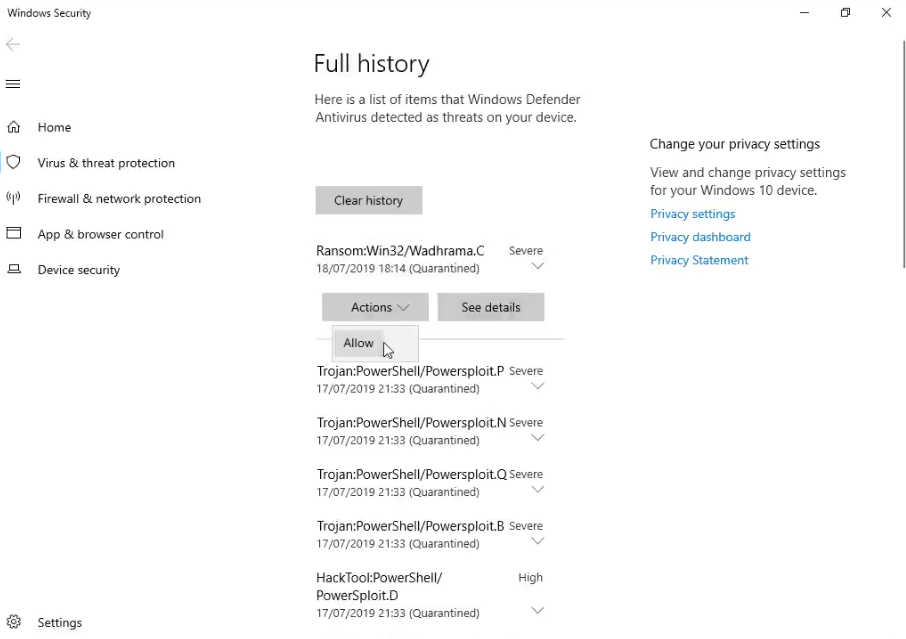
\includegraphics[width=\textwidth]{figuras/allowing_dharma_with_wd.png}
	\caption{Allowing Dharma with Windows Defender}
\end{figure}

\section*{Trobleshooting}
If running the reverse\_tcp payload with Metasploit fails to provide a Meterpreter shell is very possible that trying again ends working, because the session is not getting created even though the exploit is working.
\linej
\linej
If the integrator scripts (at least the .py scripts) are modified their changes may affect their execution by Wazuh until the \textit{wazuh-manager} service is restarted again.
\linej
\linej
Processing events can take several minutes even if the agent and manager are not under high load.
After starting a machine it is recommended to let several minutes pass before starting to do actual work.
\linej
For example real-time monitoring usually takes 3-5 minutes to report that is working in the log file.
But it can be much more if there have been unregistered changes to the monitored folders.
\linej
\linej
If you are sure that the event you want to process is being reaching the manager but no alert is being triggered, make sure that there are no rules that may be catching and silecing it with the \textit{no\_log} option or a \textit{level} option too low. If there are rules silecing the alert you must overwrite them in the custom rules using the \textit{overwrite="yes"} option in the \textit{rule} tag.
It is also important to check that there are decoders for it.
Both can be checked in the ruleset in \textit{/var/ossec/ruleset/}.
\linej
\linej
In case of suspicious connection with the agent it is recommended to check its status in the Windows machine.
This can be done with the GUI of the Wazuh agent.
The program allows to view and edit its log and configuration.
It also provides buttons to stop, start, restart and refresh its status.
\begin{figure}[H]
  \centering
	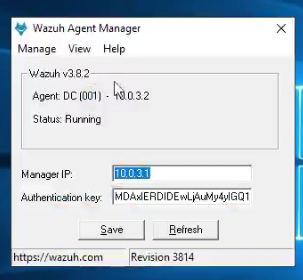
\includegraphics[width=.5\textwidth]{figuras/wazuh_agent_gui.png}
	\caption{GUI of the Wazuh agent in Windows}
\end{figure}
\linej
There can be issues with the agent even after a sucessful configuration that has been working for months.
For example due to the expiration of the registered keys or another program modifying the configuration of the agent.
